%
% File: chap01.tex
% Author: Victor F. Brena-Medina
% Description: Introduction chapter where the biology goes.
%
\let\textcircled=\pgftextcircled
\chapter{Designing the I/O Block}
\label{chap:IO_BLOCK_design}
\paragraph{}

\section{Overview}

\paragraph{}
In the previous chapter, the switch matrix was designed based on experiments run in VTR. This chapter will focus on architecting and designng the I/O Block(Input/Output Block) that will provide I/O to the FPGA fabric.

\section{I/O Block architecture}
\paragraph{}

A lot of I/O Block designs have been proposed in the academia and industry. We will try a very simple and minimal I/O block inspired from the XC2064 FPGA by Xilinx[10]. The architectural wireframe of this I/O block is shown in Fig. 5.1.

\begin{figure}[H]
\centering
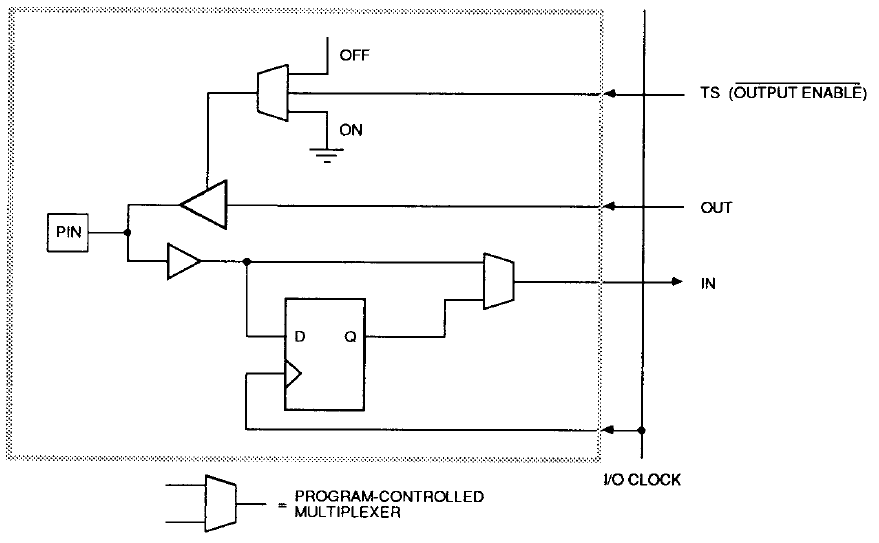
\includegraphics[width=\textwidth]{ioblock_wireframe.png}
\caption{Wireframe of the I/O Block}
\label{fig:Figure}
\end{figure}

The various components in this structure are explained below:
\begin{itemize}
\item \textbf{Input buffer : } A simple buffer using two cascaded NOT gates is used at the pin of the FPGA for receiving input from the external world. This buffer acts as a low pass filter for bouncing noise and also fixes the undershoots in HIGH / overshoots in LOW of the incoming signal.
\item \textbf{PIN :} This is the physical pin exposed to the user to apply inputs or receive outputs.
\item \textbf{D Flip-Flop :} The D Flip-Flop is used to create a registered version of the input if necessary. If an input signal in a Verilog code only appears in always@(posedge clk), then it can be registered right at its entry and can be used easily at any place required in the FPGA.
\item \textbf{2X1 Input MUX :} This MUX selects between the direct version or the registered version of the input signal.
\item \textbf{Tri-state buffer :} This buffer connects one of the neighbouring routing wires to the PIN when the I/O Block is used to send out data to the external world.
\item \textbf{3X1 tri-state control MUX :} This MUX selects whether the FPGA is sending data out to the external world or not. An output enable signal can also be used from one of the neighbouring routing wires to selectively send output at specific times.
\item \textbf{4X4 Configuration Memory :} A 16-bit SRAM arranged in a 4X4 6T-SRAM array to hold the configuration bits of the whole I/O Block. 
\begin{itemize}
\item 3-bits for selecting the output enable from one of the 4 neighbouring routing wires
\item 3-bits for selecting the output from one of the 4 neighbouring routing wires
\item 3-bits for selecting the wire where external world inputs land from the 4 neighbouring routing wires
\item 1-bit for the 2X1 Input MUX
\item 2-bits for the 3X1 tri-state control MUX
\item 2-bits for the PRE and CLR of the D Flip-Flop to determine initial state
\item 2-bits left unused for future feature updates
\end{itemize}
\end{itemize}


\section{Describing the I/O Block in VTR}
\paragraph{}
We describe our I/O block in VTR XML format and use it in the FPGA architecture used for testing. The XML description of the I/O blocks is shown in Fig. 5.2 for reference.

\begin{figure}[H]
\centering
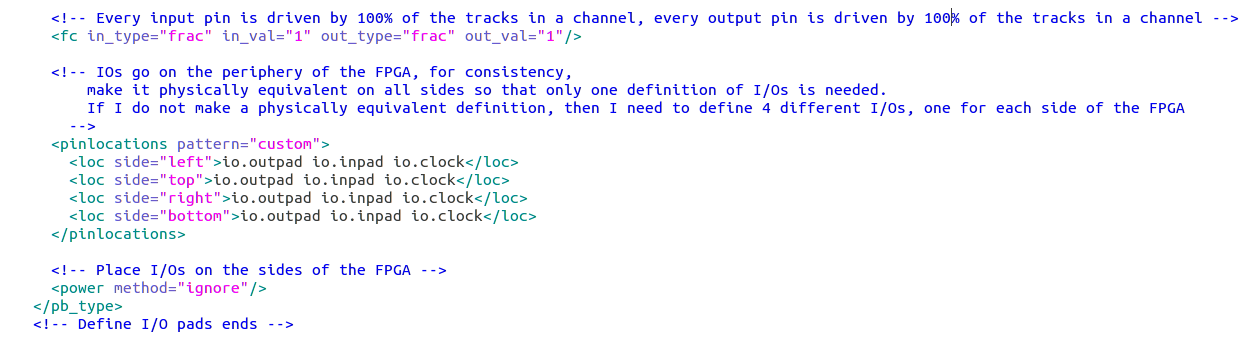
\includegraphics[width=\textwidth]{ioblockvtrdescription.png}
\caption{XML description of the I/O Block}
\label{fig:Figure}
\end{figure}


\section{Summary}
\paragraph{}
This chapter describes the architecture of the I/O block used. Each I/O block contains 16 configuration bits to program it correctly. These 16 bits are organized as a 4*4 SRAM array. The schematic of the I/O block described in Cadence Schematic L is shown in Fig. 5.3.

\begin{figure}[H]
\centering
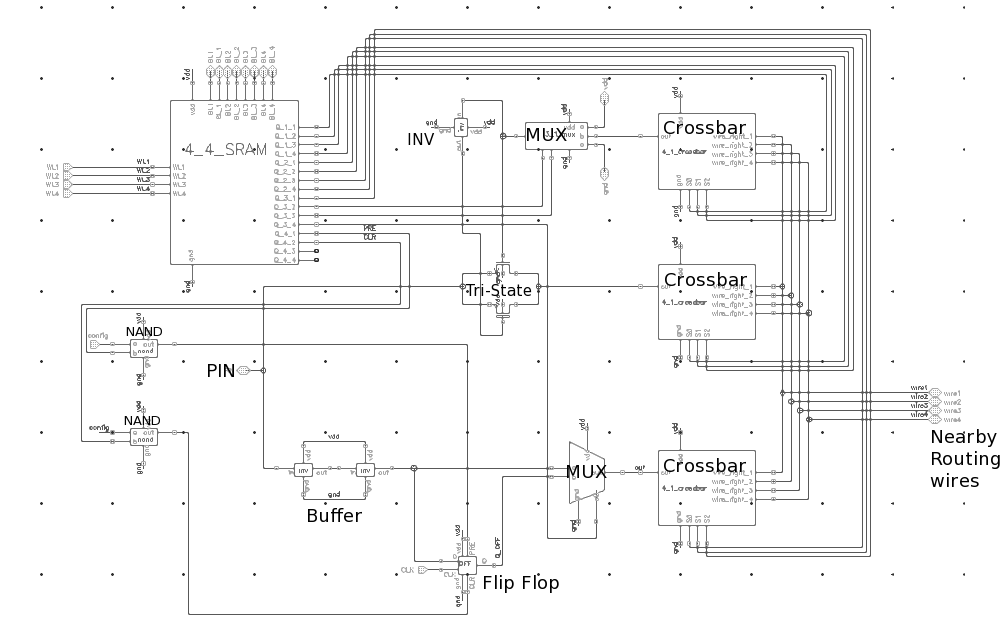
\includegraphics[width=\textwidth]{ioblock.png}
\caption{I/O Block schematic}
\label{fig:Figure}
\end{figure}


